% Chapter 3
\newcommand{\chameleon}{Chameleon}

\chapter{Chameleon: An MUS-based interactive type error visualization and explanation tool}
\label{chap:chameleon:design} 


Dynamically typed programming languages such as JavaScript and Python have risen in popularity in recent decades \cite{chatley_next_2019}. These languages present a low barrier of entry, especially to beginner programmers: they require no type declaration, variable types or object structures can be modified dynamically, and functions can deal with dynamic input using ad-hoc polymorphism and runtime reflection. However, studies show that dynamically typed languages negatively affect development productivity \cite{kleinschmager_static_2012}, code usability \cite{mayer_empirical_2012}, and code quality \cite{gao_type_2017, ray_large-scale_2017, meyerovich_empirical_2013}. They are often found to produce error-prone code \cite{chen_empirical_2020, wang_empirical_2015,xu_python_2016} and require strong programmer discipline to avoid pitfalls \cite{chen_empirical_2020}. For these reasons, many modern dynamically-typed languages have introduced static typing annotations as part of the core language features in recent years (e.g.\ \textit{TypeScript}~\cite{microsoft_javascript_nodate} and \textit{mypy}~\cite{mypy_mypy_nodate}).

Functional programming languages have long enjoyed rigorous type systems and expressive type-level features. Techniques such as type inference and algebraic types have been standard practice for decades in functional languages such as ML and Haskell, and more recently in multi-paradigm languages, such as Rust and TypeScript. Various type system advances were introduced in Haskell and ended up in mainstream languages years or even decades after, leading many to consider Haskell the ``type-system laboratory" \cite{hudak_history_2007}.  Type classes, an implementation of generic programming, were introduced to Haskell in 1988~\cite{hudak_history_2007}, and now can be found in most popular languages such as C\#~\cite{bill_wagner_constraints_2022}, Java~\cite{oracle_generic_2022}, and TypeScript~\cite{microsoft_documentation_2022}.

One crucial challenge of programming in statically-typed languages is that type errors can sometimes be difficult to resolve~\cite{tirronen_understanding_2015, hage_solved_2020}. In particular, they may point to locations that are not the root  causes of the type error, expose errors in cryptic language, or provide misleading fixing suggestions~\cite{wu_how_2017}.


\section{Motivation Example}

The design requirements of \chameleon{} are motivated by limitations of traditional type errors, as documented in a number of studies (e.g.~\cite{yang_improved_2000, hage_solved_2020}), but which we illustrate here with a few motivating examples. 

\begin{figure}
    \centering
    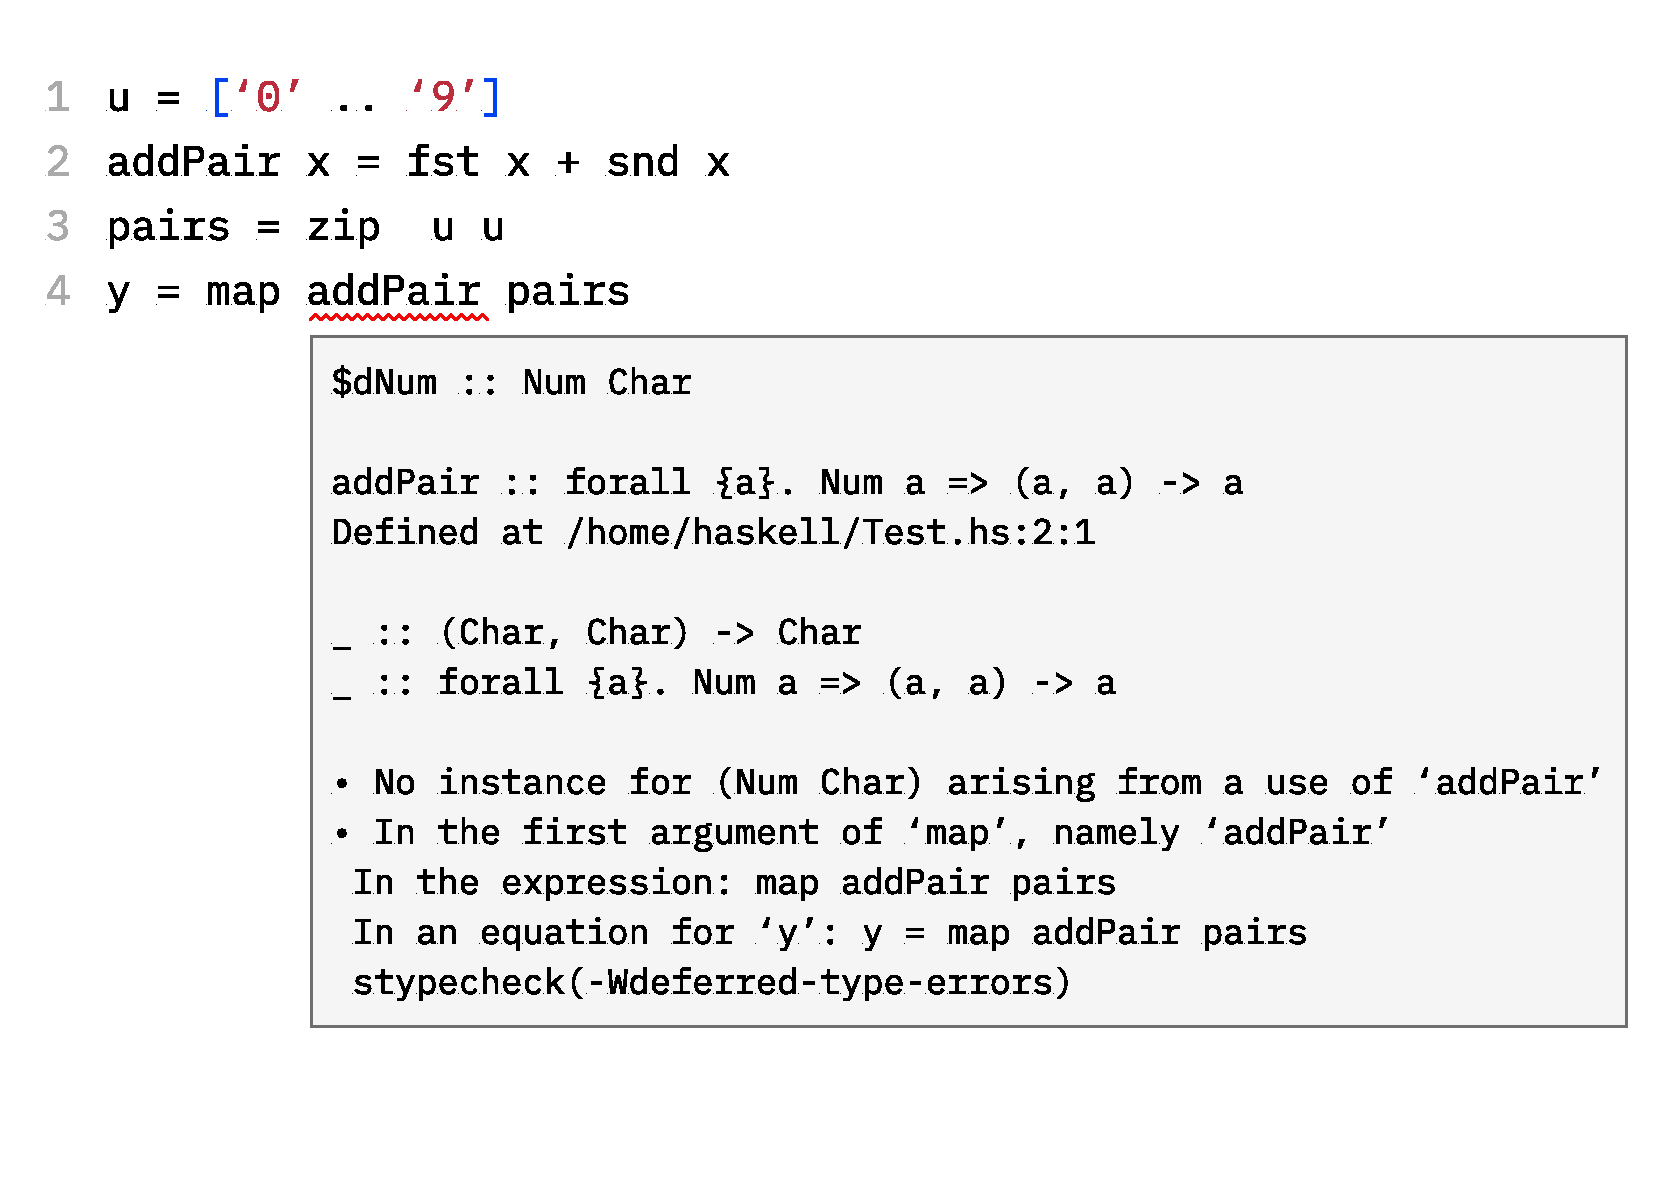
\includegraphics[width=\linewidth,trim=0mm 35mm 0mm 0mm]{Figures/add-pair-example.pdf}
    \caption{
    A type error displayed in Visual Studio Code\cite{microsoft_visual_nodate} and the Haskell Vscode extension~\cite{haskell_haskell_nodate}.
The expression \texttt{addPair} is blamed for causing the type error. This may not match the programmers' intention. 
    }
    \label{fig:motivation-example}
\end{figure}

\subsubsection{\textbf{Traditional type errors show only limited location}}
Haack and Wells~\cite{haack_type_2004} noted that ``\textit{Identifying only one node or subtree of the program as the error location makes it difficult for programmers to understand type errors. To choose the correct place to fix a type error, the programmer must find all the other program points that participate in the error.}'' The type error in Fig.~\ref{fig:motivation-example} can be fixed in multiple locations. For instance  replacing \texttt{['0'..'9']} on line 1 with \texttt{[0..9]}, or replacing \texttt{fst x} and \texttt{snd x} on line 2 with \texttt {read (fst x)} and \texttt{read (snd  x)}. In the type error message, only the \texttt{addPair} expression on line 4 was blamed.  In this small example, the whole context is visible, but it can become problematic in large programs where the lines contributing to the type error are far apart in the source code.

\subsubsection{\textbf{Traditional type errors are biased}}
A common form of bias happens when a type error is reported in one expression, but it can occur in multiple other expressions as well. In Fig.~\ref{fig:motivation-example}, the error message arbitrarily focuses on only \texttt{addPair}, while ignoring that the literals in the definition of \texttt{u} may be incorrect. 

Another form of bias is that traditional type errors are often framed as conflicts between \texttt{Expected type} and \texttt{Actual type}. This framing is standard practice in most typed languages. However, what is \texttt{expected} and what is \texttt{actual} are a side effect of different unification orders rather than the intention of the programmer. In both forms, the error message may lead programmers to falsely believe the validity of parts of code and wrongly accuse others.

\subsubsection{\textbf{Traditional type errors give poor explanations}}
When the compiler rejects a program, the internal state of type checking is the result of a complex computation. But the details of this process are hard to explain to users and are usually not reported by compilers. For the typical type error shown in Fig.~\ref{fig:motivation-example}, the evidence for the type error is gathered from the previous declarations. These have to be rediscovered by programmers using less rigorous methods. 

\subsection{Design Goals of \chameleon{}}
Based on the limitations of traditional type errors, we give the following design requirements for \chameleon{}:

\noindent\textbf{Show} all the possible locations where the type error happened or could have happened.

\noindent\textbf{Explain} type errors avoiding jargon and internal constructs of the type checker.

\noindent\textbf{Do not presume} which expression is to blame for the type error based on the order of computation or which possible type for an expression is `actual' or `expected'.


\section{Features of Chameleon}

Discuss the features of Chameleon, different debugging utilities and modes.

\section{Implementation}

Discuss the implementation of Chameleon. 

\section{Walkthrough}

Explain the interactive features of Chameleon via a semi-realistic debugging example.

\section{Conclusion}
